\documentclass[]{IEEEphot}

\jvol{xx}
\jnum{xx}
\jmonth{June}
\pubyear{2015}

\newtheorem{theorem}{Theorem}
\newtheorem{lemma}{Lemma}

\begin{document}

\title{Olympic Ski Jump Design}

\author{Raul~E.~Jordan, Ha~Le,
\\
Deven~Hurt, Maille~Radford}

\affil{Harvard University Physical Sciences \& 12a
Final Project Report\\ Cambridge, MA}  

\doiinfo{PS12a Final Project Report Using\\
Matlab for Numerical Analysis 2015 Harvard College}%

\maketitle


\begin{receivedinfo}
\begin{center}
Statement of Problem: To design a model for an olympic ski jump and to determine the best angles for the mountain and ski jump ramp to maximize distance traveled.
\end{center}
\end{receivedinfo}

\begin{abstract}
 The goal of this final project is to determine the ideal angle of a ski jump in order to maximize the distance that the skier travels before landing down the mountain.

\end{abstract}

\section{Hypothesis}
 In order to maximize the skier’s velocity as he leaves the ramp, the angle of the mountain should be greater than that of the ramp. This will allow him to accelerate down the mountain and reach a greater velocity before traveling up the ramp. As the ramp slopes upward, this will decrease his velocity; by reducing the angle of the ramp, therefore, we may reduce this effect by decreasing the magnitude of the forces acting upon the skier in the opposite direction. According to the International Ski Federation, the angle of the mountain must be between 30 and 37 (Gasser 8). We hope, therefore, to find a best  for the mountain within this range. Additionally, the angle of the ramp relative to the horizontal should be between 8 and 12 (Gasser 15).

 \section{Assumptions}
 To simplify the problem, we assumed that $\theta_1$ would be the angle for the downslide portion of the ski jump design and the mountain in our variables
\
 We also assumed that the bend of the mountain could be represented by a parabolic function, which we eventually used when calculating the distance by finding the arc length of this function.
\
 We considered the person to be a cylinder so that their cross-sectional area was a rectangle equal to $2rL$
 where
 	r = the ``radius'' of the person, assumed to go from the middle of the chest to the shoulder, which is approximately 0.23m by analyzing the average width of a man from shoulder to shoulder

	L = his height, or L, is 1.8m (an assumed value for the height of the man)
\
In part I of our model, the skier is crouched; therefore, we determined that L would be $\frac{1.8m}{2}$
In part II, the skier extends to his full height, $1.8$m , when in the air
We assumed that the skier’s mass was $70$ kg



\section{Procedure}

Before using Matlab, we drew the mountain and ramp system and identified variables within this. From this diagram, we decided to divide our calculations into two parts: the skier in contact with the mountain and ramp and the projectile motion of the skier when leaving the ramp.

\subsection{Part I: Skier in Contact with the Mountain and Ramp}

There are three portions of the skier’s descent down the mountain: the downward linear path of the mountain, the parabolic bend of the mountain, and the upward linear ski jump. In setting up the calculations for this first part, we, therefore, divided the problem into three subsections.

When traveling down the linear portion of the mountain, the skier is experiencing four forces--the gravitational force, normal force from the mountain, kinetic friction, and drag due to air resistance. Because he is not simply experiencing normal and gravitational forces, his initial gravitational potential energy is converted to both kinetic energy and thermal energy. Using the Conservation of Energy and assuming that the skier has an initial velocity of $0 m/s$, we may set up the equation:

\[
	U_g = K + E_th \rightarrow \frac{1}{2}mgh_1 + \mu_k mgcos\theta_1 \frac{h_1}{sin\theta_1} + \frac{1}{2}C_d\rho Av^2 \frac{h_1}{sin\theta_1}   \ \         (eq 1)
\]

With the height of the mountain, $h_1$, $U_g = mgh$ and $K = \frac{1}{2} mgh_1$. The thermal energy, $E_th$, includes two components, that due to drag and to kinetic friction. To calculate these two components, we multiplied the distance traveled, $\frac{h}{sin\theta_1}$, ($\theta_1$ is the angle of the mountain)  by the force of drag and the force of friction, respectively. $v_1$, the velocity at the end of the linear segment of the mountain, was found to be:

\[
	v_1 = \sqrt{\frac{2mgh_1 - 2\mu_k mgcos\theta_1 \frac{h_1}{sin\theta_1}}{m + C_d\rho A\frac{h_1}{sin\theta_1}}} \ \ (eq 2)
\]

The skier then moves onto the bend in the mountain, which could be represented by circle, parabola, or hyperbolic cosine functions. We decided to represent this distance, $L_{other}$ (to distinguish it from the L used as the height of the person), by the parabolic function:

\begin{eqnarray}
f = \frac{h_2}{tan\theta_1}\nonumber\\
x = \frac{h_1}{sin\theta_1} \nonumber\\
L_{other} = \int_0^f \frac{h_2}{\sqrt{1 + 4x^2}} dx \ \ (eqn 3) \nonumber
\end{eqnarray}

The skier is still experiencing the same four forces. Therefore, with this parabolic model, the equation for $v_1$ can be modified to find the velocity at the base of the parabola, $v_2$:

\[
	v_2 = \sqrt{\frac{2mgh_2 - 2\mu_k mgcos\theta_2 \left|L_{other}\right| }{C_d\rho A\frac{h_1}{sin\theta_1}}} + v_1\ \ (eq 4)
\]

As seen in (eqn 4), the initial velocity in calculating $v_2$ cannot be assumed to be $0 m/s$ as in (eqn 2); rather, $v_1$ is added as the initial velocity to give the skier’s total velocity just before reaching the ramp.

When on the ramp, the direction of the normal force, kinetic friction, and drag rotate to the left by $90\deg$ the ramp now slopes upward (see fig. 2b). This change in the forces applied to the skier causes his velocity to decrease as he moves up the ramp because these forces result in a negative acceleration. Using the Conservation of Energy once more:



\subsection{Part II: Projectile Motion of the Skier After Leaving the Ramp}

After leaving the ramp with a velocity $v_3$, the skier follows a trajectory through the air with projectile motion. As he is no longer in contact with the mountain or ramp, he does not experience normal force or kinetic friction; the only forces acting upon him, therefore, are drag and gravitational force. Previously, when the skier was traveling down the mountain and upward along the ramp, he was in a crouched position to reduce drag and increase his velocity. We assumed that he was half of his standing height at this time. When leaving the ramp, however, we have observed that ski jumpers extend to their full height but travel with their bodies angled towards the ground rather than perpendicular. This helps to reduce their surface area and, therefore, drag.

Having run the MATLAB code to determine the best $\theta_1$ and $\theta_2$ of the mountain and ramp, respectively, we may determine how far the skier is able to jump before hitting the mountain. We first determined the maximum distance traveled along the $x$-axis if the surface had been horizontal. As the mountain slopes downward, we then used this distance and the best angle of the mountain, $\theta_1$, to determine the distance traveled relative to the mountain. This is found by determining when the the slope of the mountain intersects with the position of the skier.


\section{Analysis and Conclusions}

Placing the model equations derived into the MATLAB and using a for-loop and evolver from HW7 to find the best value of our system, we found the best angles for our ski jump design and the resulting distance that the skier is able to reach. The ideal angle for the mountain would be $31.414$ degrees; the ideal angle for the ramp would be $11.414$ degrees. Having angles greater than the ideal ones would result in a decrease in velocity for the ski jumper (as represented in Graph 1), thus directly correlating with a decrease in distance traveled. Utilizing such a ski jump design and considering the assumptions we made, the skier would be able to travel $68.964$ m from take-off at the end of the ramp. The angles determined through our final project falls within the range of those deemed the best by International Ski Federation; thus, this indicates that we were able to successfully create a model that gave realistic angles for the design. Furthermore, the International Ski Federation calculated that the velocity leaving the ramp would have to be $17.5 m/s$ (Gasser 18); the take-off velocity that our model gave us was $16.0368 m/s$; therefore, our model is consistent with actual ski jumps. Thus, in general, our application of knowledge concerning kinematics and dynamics was successful and we were able to use MATLAB to design a ski jump that would maximize the distance traveled by the skier.

\section{Acknowledgements}
We would like to thank Professor Kaxiras Nils and Joon for their immense help this semester. 


\section{References}
Gasser, Hans-Heini (2012). “Standards for the construction of jumping hills - 2012.” Federation internationale du ski. Oberhofen: FIS.
\\
Müller, Wolfram (2005). “The physics of ski jumping.” Proceedings of European School of High-Energy Physics. Geneva: CERN. pp. 269–278.



\begin{figure}
\centering%
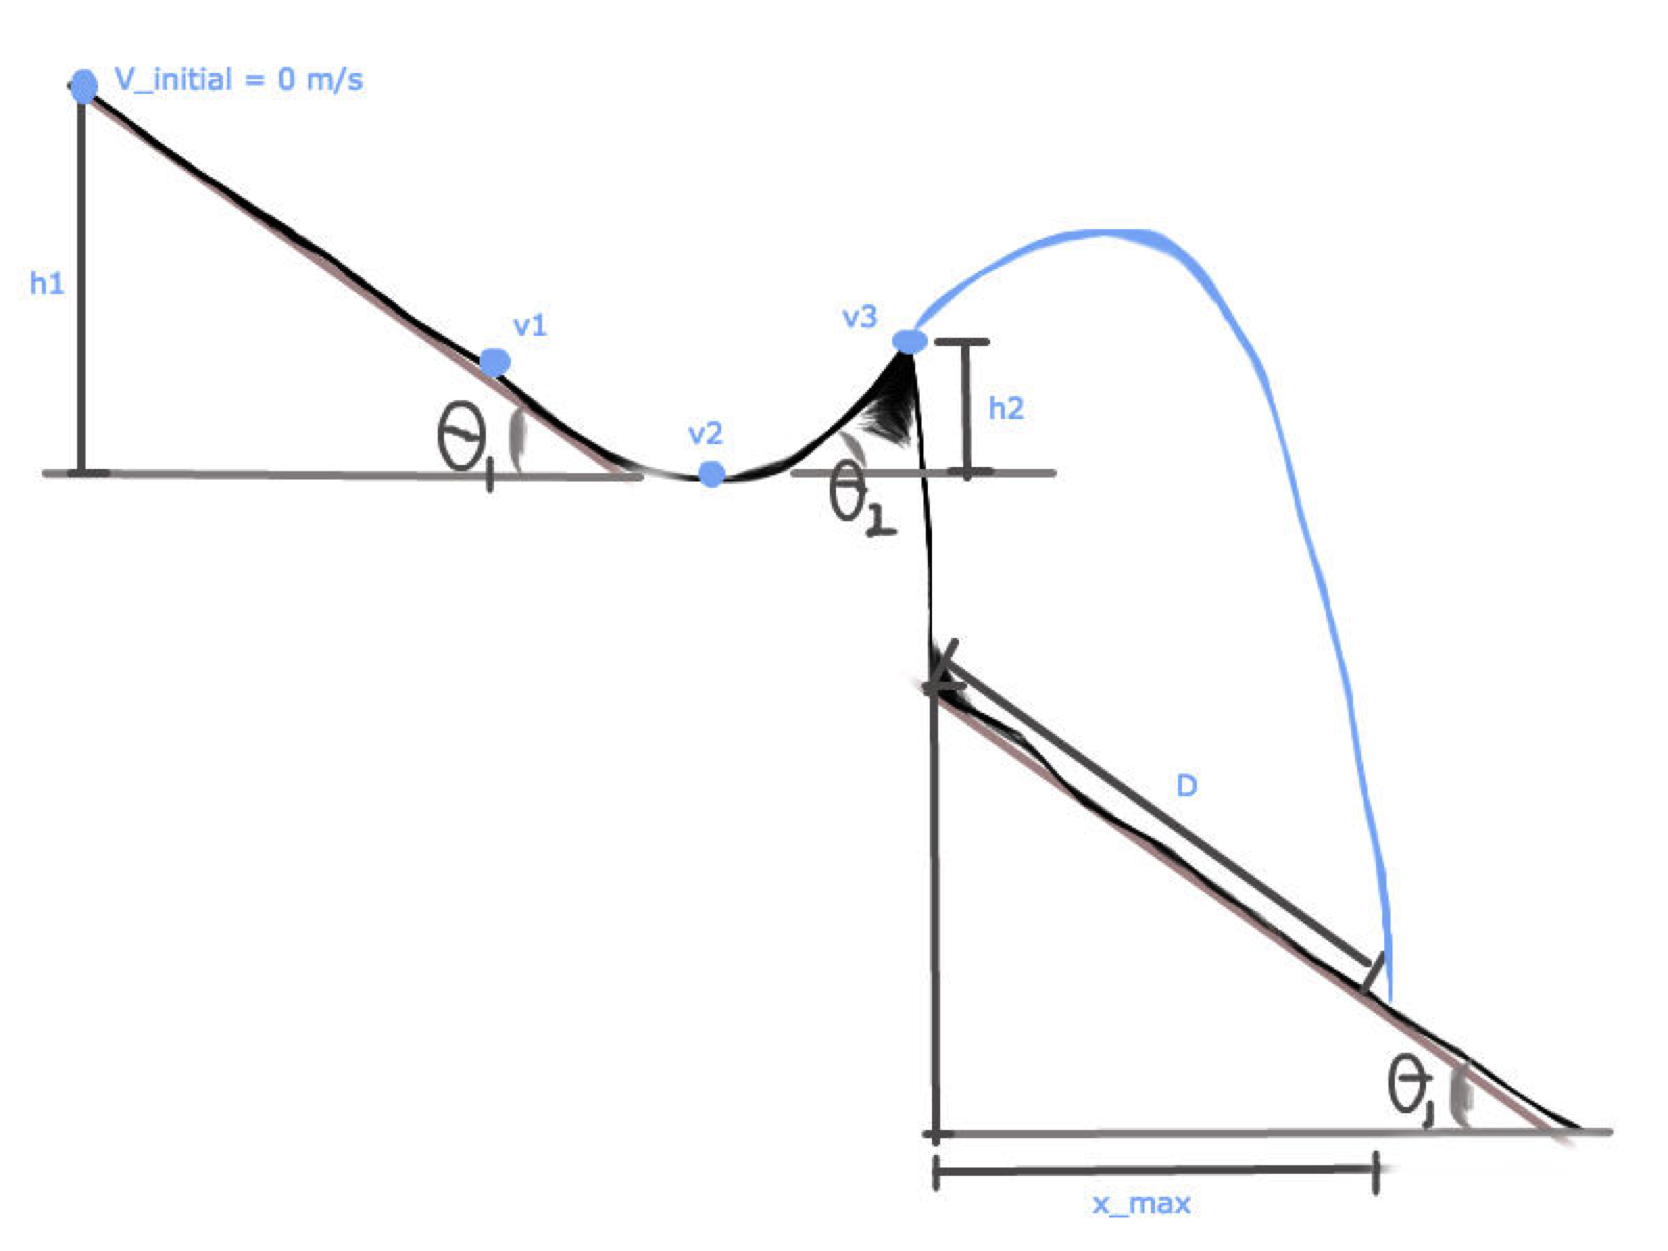
\includegraphics[width=21pc]{ramp}
\caption{This is the diagram we used to write our model equations. Here: $v_initial$ is the velocity that the ski jumper begins with at the top of the mountain; $v1$ is the velocity at the end of the jumper’s downward descent down the mountain ramp; $v2$ is the velocity of the jumper at the apex of the ramp; $v3$ is the take-off velocity of the jumper; $h1$ is the height of the ski jumper before his descent in relation to the horizontal; $h2$ is the height of the ski jumper at the point of his take-off in relation to the horizontal; $x_max$ is the maximum distance he travels in the x-direction; D is the maximum distance that the ski jumper travels in general after take-off; 1 is the angle of the mountain; and 2 is the angle of the ramp.}
\label{fig1}
\end{figure}

\begin{figure}
\centering%
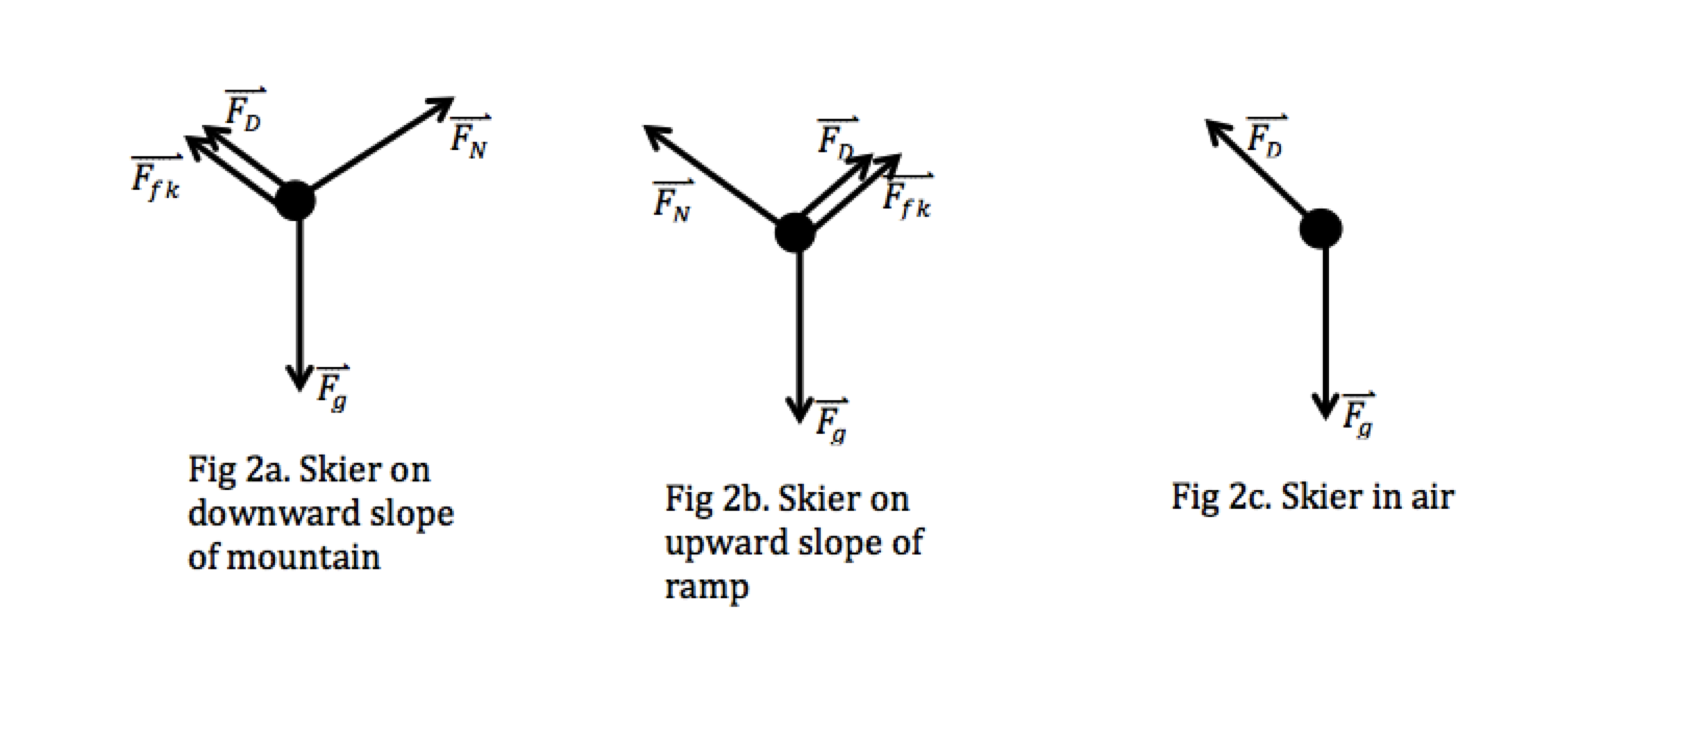
\includegraphics[width=21pc]{force}
\caption{Force diagrams for the ski jumper at different points in his jump.}
\label{fig2}
\end{figure}

\begin{figure}
\centering%
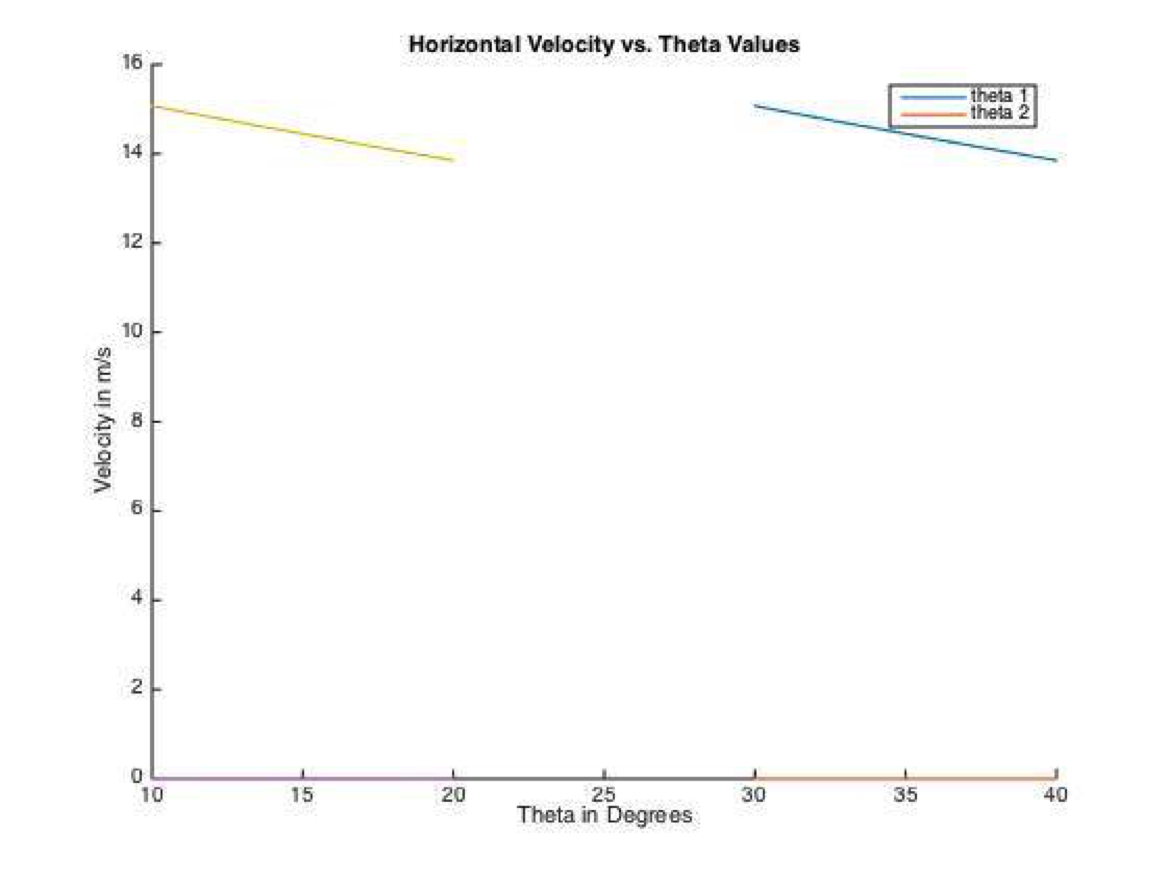
\includegraphics[width=21pc]{graph1}
\caption{ Horizontal Velocity vs. Theta Velocities}
\label{fig3}
\end{figure}

\begin{figure}
\centering%
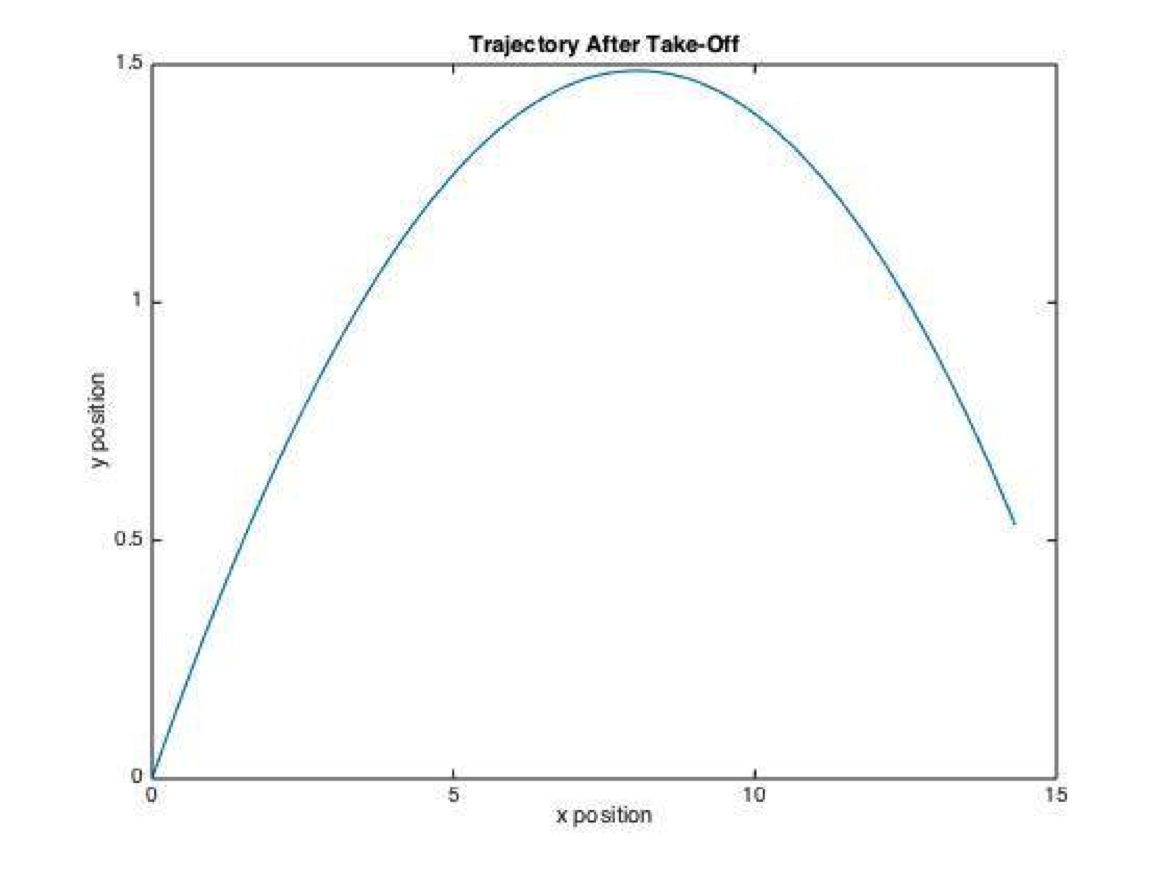
\includegraphics[width=21pc]{graph2}
\caption{ The trajectory of the ski jumper in our best fit model after take-off }
\label{fig4}
\end{figure}



\end{document}
